\capitulo{4}{Técnicas y herramientas}

Esta parte de la memoria tiene como objetivo presentar las técnicas metodológicas y las herramientas de desarrollo que se han utilizado para llevar a cabo el proyecto.

\section{Herramientas utilizadas}
\begin{itemize}
\item Python: Python es un lenguaje de programación de alto nivel ampliamente utilizado en el campo del aprendizaje automático y la inteligencia artificial. Posee una gran catidad de bibliotecas y frameworks que facilitan el procesamiento de datos y la implementación de algoritmos de inteligencia artificial.
En este proyecto ha sido utilizado para desarrollar toda la parte del back-end de la aplicación. 

\item librosa: librosa es una biblioteca de Python utilizada para el análisis y procesamiento de audio. Proporciona una amplia gama de métodos para extraer características de audio de forma sencilla. Algunos ejemplos son espectrogramas, coeficientes cepstrales de frecuencia mel (MFCC) o cromagramas.
En este proyecto ha sido utilizada para procesar y extraer diversas características de audio para alimentar los algoritmos de inteligencia artificial y crear el modelo.

\item TensorFlow: TensorFlow es una biblioteca de código abierto utilizada en el campo del aprendizaje automático. Proporciona una interfaz sencilla para la implementación de redes neuronales y otros algoritmos de aprendizaje automático.
TensorFlow ha sido la opción escogida para entrenar los algoritmos de redes neuronales del proyecto.

\item scikit-learn: scikit-learn es una biblioteca de aprendizaje automático de Python que proporciona una amplia gama de algoritmos y herramientas para el análisis de datos y la construcción de modelos. Incluye funciones para la división de conjuntos de datos en conjuntos de entrenamiento (\textit{train} y \textit{prueba}).

\item NumPy: NumPy es una biblioteca de Python utilizada para realizar cálculos numéricos en matrices y matrices multidimensionales. Proporciona una amplia gama de funciones matemáticas y herramientas para el manejo eficiente de datos numéricos.

\item Pandas: bibliteca de código abierto en Python que proporciona herramientas de análisis de datos. Es ampliamente usada en el mundo de la ciencia de datos.
\end{itemize}

\section{Justificación}

\subsection{Python}
A continuación se presentan algunas justificaciones que han decantado el desarrollo del proyecto en lenguaje Python en comparación con otros lenguajes de programación.

\textbf{Amplia variedad de bibliotecas y frameworks}: Python cuenta con una amplia gama de bibliotecas y frameworks especializados en aprendizaje automático, como TensorFlow, scikit-learn, PyTorch, Keras y muchos otros. 
Estas bibliotecas proporcionan herramientas e implementación de los principales algoritmos de inteligencia artificial, lo que facilita enormemente la tarea de desarrollar un proyecto de aprendizaje automático.

\textbf{Integración con otras tecnologías}: Python se integra fácilmente con otras tecnologías existentes en el ámbito del desarrollo del aprendizaje automático. Por ejemplo, se puede combinar con bases de datos (MySQL), herramientas de visualización (matplotlib), análisis de datos (Pandas) o en este caso herramientas de procesamiento musical (librosa).

\subsection{TensorFlow vs scikit-learn}
La elección de utilizar TensorFlow en lugar de scikit-learn se basa en varias consideraciones.

\textbf{En primer lugar}, TensorFlow es adecuado para proyectos que involucran aprendizaje profundo y redes neuronales. Proporciona una mayor cantidad de herramientas para crear, entrenar y desplegar modelos de aprendizaje profundo que scikit-learn. 

\textbf{TensorFlow} permite implementar arquitecturas de redes neuronales complejas, como redes neuronales convolucionales (CNN), las cuales son muy adecuadas para los objetivos del proyecto.

\textbf{Por último}, TensorFlow tiene soporte para utilizar tarjetas gráficas (GPUs) a la hora de realizar el proceso de entrenamiento. Esto proporciona una ventaja significativa en rendimiento, ya que al poder utilizar la gran cantidad de nucleos de una GPU se pueden realizar cálculos de manera paralela y distribuida lo que resulta en tiempos
de entrenamiento considerablemente más rápidos en comparación con el uso exclusivo de CPU.

\section{Técnicas utilizadas}

Se han utilizado diversas técnicas y metodologías para llevar a cabo el desarrollo y entrenamiento de los modelos de aprendizaje automático.

(En el documento \textit{Anexos} se describe de una forma mucho más profunda el desarrollo metodológico del proyecto.)

\section{Procesamiento y extracción de características de audio}

Para el procesamiento y extracción de características de audio, se ha utilizado la biblioteca librosa en Python.

\begin{itemize}
\item MFCC (coeficientes cepstrales de frecuencia mel): Estos coeficientes capturan las características espectrales del audio y se utilizan comúnmente en tareas de reconocimiento de voz y clasificación de audio. Son las características principales que se han utilizado para entrenar el modelo y realizar predicciones.
\end{itemize}

\section{División del conjunto de datos}

Para dividir el conjunto de datos en conjuntos de entrenamiento, prueba y validación, se ha utilizado la biblioteca scikit-learn. 
Scikit-learn proporciona una función llamada \textit{train\textunderscore test\textunderscore split} que permite dividir el conjunto de datos en partes destinadas para el entrenamiento y la evaluación del modelo. Esta técnica de división del conjunto de datos es fundamental para evaluar la capacidad de \textbf{generalización} del modelo y evitar el \textbf{sobreajuste}.

\begin{figure}
  \centering
  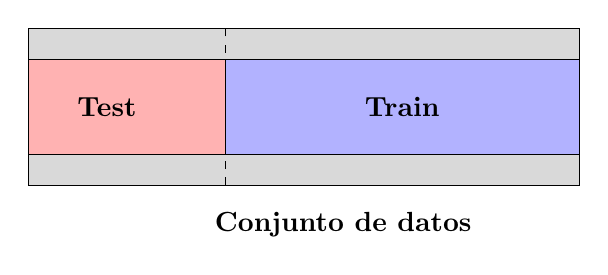
\begin{tikzpicture}
    % Ancho de los conjuntos de entrenamiento y prueba
    \def\datasetwidth{6}
    
    % dataset
    \draw[fill=gray!30] (-1,0) rectangle (\datasetwidth,2);
    
    % test
    \draw[fill=red!30] (-1,0.4) rectangle (1.5,1.6);
    \node at (0,1) {\textbf{Test}};
    
    % train
    \draw[fill=blue!30] (1.5,0.4) rectangle (\datasetwidth,1.6);
    \node at (3.75,1) {\textbf{Train}};
    
    \draw[dashed] (1.5,0) -- (1.5,2);
    
    \draw[dashed] (-1,0.4) -- (\datasetwidth,0.4);
    \draw[dashed] (-1,1.6) -- (\datasetwidth,1.6);
    
    % Etiqueta del conjunto completo
    \node at (\datasetwidth/2,-0.5) {\textbf{Conjunto de datos}};
  \end{tikzpicture}
  \caption{División del conjunto de datos}
\end{figure}

\section{Redes neuronales con TensorFlow}

Para realizar el entrenamiento de los datos, se han utilizado redes neuronales implementadas con la biblioteca TensorFlow.

En este proyecto, se han utilizado diferentes arquitecturas de redes neuronales, como redes neuronales convolucionales (CNN) y redes neuronales multicapa. Estas arquitecturas son adecuadas para tareas de procesamiento de audio y han demostrado ser efectivas en la clasificación y reconocimiento de patrones en audio.

Las redes neuronales se entrenan actualizando los pesos y los sesgos de la red iterativamente para minimizar la pérdida (\textit{loss}). Una vez entrenadas, las redes neuronales realizan predicciones sobre nuevos datos de audio, clasificándolos en categorías o estilos musicales.

\begin{figure}
  \centering
  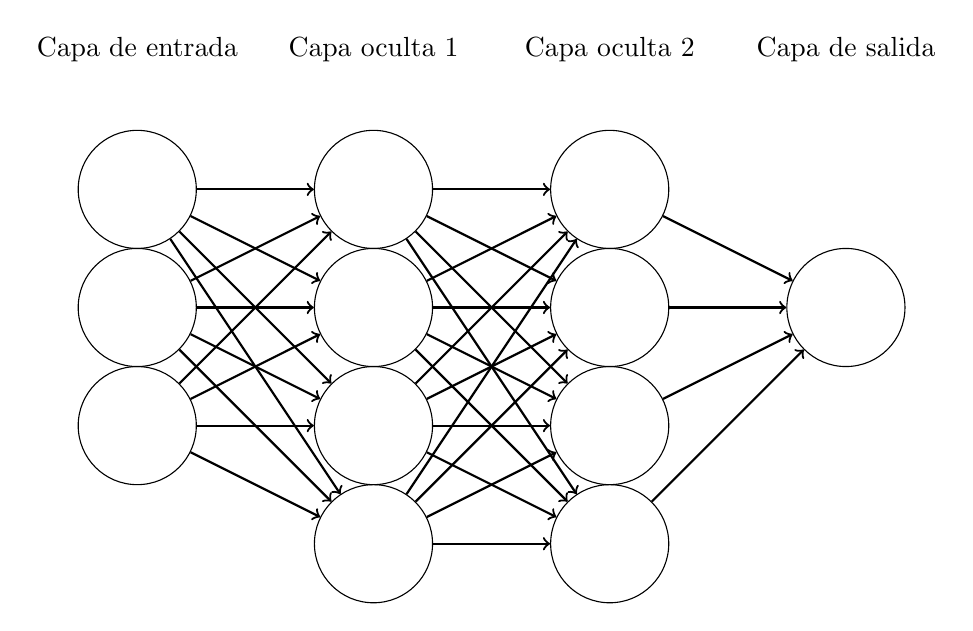
\begin{tikzpicture}[
    neuron/.style={circle, draw, minimum size=1.5cm},
    connection/.style={->, thick}
  ]
    % Input layer
    \foreach \i in {1,2,3}
      \node[neuron] (input\i) at (0,-\i*1.5) {};

    % Hidden layer 1
    \foreach \i in {1,2,3,4}
      \node[neuron] (hidden1\i) at (3,-\i*1.5) {};

    % Hidden layer 2
    \foreach \i in {1,2,3,4}
      \node[neuron] (hidden2\i) at (6,-\i*1.5) {};

    % Output layer
    \node[neuron] (output) at (9, -3) {};

    % Connections
    \foreach \i in {1,2,3}
      \foreach \j in {1,2,3,4}
        \draw[connection] (input\i) -- (hidden1\j);

    \foreach \i in {1,2,3,4}
      \foreach \j in {1,2,3,4}
        \draw[connection] (hidden1\i) -- (hidden2\j);

    \foreach \i in {1,2,3,4}
      \draw[connection] (hidden2\i) -- (output);

    \node[above] at (0,0) {Capa de entrada};
    \node[above] at (3,0) {Capa oculta 1};
    \node[above] at (6,0) {Capa oculta 2};
    \node[above] at (9,0) {Capa de salida};

  \end{tikzpicture}
  \caption{Ejemplo de una red neuronal multicapa}
\end{figure}

\section{Desarrollo con Python y Flask}

La parte del desarrollo de la aplicación web se ha llevado a cabo utilizando Python y el framework Flask. Flask es un framework web que permite construir aplicaciones web en Python.

Utilizando Flask, se ha desarrollado el back-end de la aplicación, que se encarga de recibir las solicitudes del usuario, procesar los datos de audio y devolver los resultados de clasificación y análisis. Todo ello mediante la implementación de RESTful API, lo que proporciona una comunicación contínua entre el usuario y el servidor.

